\PassOptionsToPackage{unicode=true}{hyperref} % options for packages loaded elsewhere
\PassOptionsToPackage{hyphens}{url}
%
\documentclass[
  ,man,floatsintext]{apa6}
\usepackage{lmodern}
\usepackage{amssymb,amsmath}
\usepackage{ifxetex,ifluatex}
\ifnum 0\ifxetex 1\fi\ifluatex 1\fi=0 % if pdftex
  \usepackage[T1]{fontenc}
  \usepackage[utf8]{inputenc}
  \usepackage{textcomp} % provides euro and other symbols
\else % if luatex or xelatex
  \usepackage{unicode-math}
  \defaultfontfeatures{Scale=MatchLowercase}
  \defaultfontfeatures[\rmfamily]{Ligatures=TeX,Scale=1}
\fi
% use upquote if available, for straight quotes in verbatim environments
\IfFileExists{upquote.sty}{\usepackage{upquote}}{}
\IfFileExists{microtype.sty}{% use microtype if available
  \usepackage[]{microtype}
  \UseMicrotypeSet[protrusion]{basicmath} % disable protrusion for tt fonts
}{}
\makeatletter
\@ifundefined{KOMAClassName}{% if non-KOMA class
  \IfFileExists{parskip.sty}{%
    \usepackage{parskip}
  }{% else
    \setlength{\parindent}{0pt}
    \setlength{\parskip}{6pt plus 2pt minus 1pt}}
}{% if KOMA class
  \KOMAoptions{parskip=half}}
\makeatother
\usepackage{xcolor}
\IfFileExists{xurl.sty}{\usepackage{xurl}}{} % add URL line breaks if available
\IfFileExists{bookmark.sty}{\usepackage{bookmark}}{\usepackage{hyperref}}
\hypersetup{
  pdftitle={Simulation-Based Power-Analysis for Factorial ANOVA Designs},
  pdfauthor={Daniël Lakens~\& Aaron R. Caldwell},
  pdfkeywords={power analysis, ANOVA, hypothesis test, sample size justification, repeated measures},
  pdfborder={0 0 0},
  breaklinks=true}
\urlstyle{same}  % don't use monospace font for urls
\usepackage{color}
\usepackage{fancyvrb}
\newcommand{\VerbBar}{|}
\newcommand{\VERB}{\Verb[commandchars=\\\{\}]}
\DefineVerbatimEnvironment{Highlighting}{Verbatim}{commandchars=\\\{\}}
% Add ',fontsize=\small' for more characters per line
\usepackage{framed}
\definecolor{shadecolor}{RGB}{248,248,248}
\newenvironment{Shaded}{\begin{snugshade}}{\end{snugshade}}
\newcommand{\AlertTok}[1]{\textcolor[rgb]{0.94,0.16,0.16}{#1}}
\newcommand{\AnnotationTok}[1]{\textcolor[rgb]{0.56,0.35,0.01}{\textbf{\textit{#1}}}}
\newcommand{\AttributeTok}[1]{\textcolor[rgb]{0.77,0.63,0.00}{#1}}
\newcommand{\BaseNTok}[1]{\textcolor[rgb]{0.00,0.00,0.81}{#1}}
\newcommand{\BuiltInTok}[1]{#1}
\newcommand{\CharTok}[1]{\textcolor[rgb]{0.31,0.60,0.02}{#1}}
\newcommand{\CommentTok}[1]{\textcolor[rgb]{0.56,0.35,0.01}{\textit{#1}}}
\newcommand{\CommentVarTok}[1]{\textcolor[rgb]{0.56,0.35,0.01}{\textbf{\textit{#1}}}}
\newcommand{\ConstantTok}[1]{\textcolor[rgb]{0.00,0.00,0.00}{#1}}
\newcommand{\ControlFlowTok}[1]{\textcolor[rgb]{0.13,0.29,0.53}{\textbf{#1}}}
\newcommand{\DataTypeTok}[1]{\textcolor[rgb]{0.13,0.29,0.53}{#1}}
\newcommand{\DecValTok}[1]{\textcolor[rgb]{0.00,0.00,0.81}{#1}}
\newcommand{\DocumentationTok}[1]{\textcolor[rgb]{0.56,0.35,0.01}{\textbf{\textit{#1}}}}
\newcommand{\ErrorTok}[1]{\textcolor[rgb]{0.64,0.00,0.00}{\textbf{#1}}}
\newcommand{\ExtensionTok}[1]{#1}
\newcommand{\FloatTok}[1]{\textcolor[rgb]{0.00,0.00,0.81}{#1}}
\newcommand{\FunctionTok}[1]{\textcolor[rgb]{0.00,0.00,0.00}{#1}}
\newcommand{\ImportTok}[1]{#1}
\newcommand{\InformationTok}[1]{\textcolor[rgb]{0.56,0.35,0.01}{\textbf{\textit{#1}}}}
\newcommand{\KeywordTok}[1]{\textcolor[rgb]{0.13,0.29,0.53}{\textbf{#1}}}
\newcommand{\NormalTok}[1]{#1}
\newcommand{\OperatorTok}[1]{\textcolor[rgb]{0.81,0.36,0.00}{\textbf{#1}}}
\newcommand{\OtherTok}[1]{\textcolor[rgb]{0.56,0.35,0.01}{#1}}
\newcommand{\PreprocessorTok}[1]{\textcolor[rgb]{0.56,0.35,0.01}{\textit{#1}}}
\newcommand{\RegionMarkerTok}[1]{#1}
\newcommand{\SpecialCharTok}[1]{\textcolor[rgb]{0.00,0.00,0.00}{#1}}
\newcommand{\SpecialStringTok}[1]{\textcolor[rgb]{0.31,0.60,0.02}{#1}}
\newcommand{\StringTok}[1]{\textcolor[rgb]{0.31,0.60,0.02}{#1}}
\newcommand{\VariableTok}[1]{\textcolor[rgb]{0.00,0.00,0.00}{#1}}
\newcommand{\VerbatimStringTok}[1]{\textcolor[rgb]{0.31,0.60,0.02}{#1}}
\newcommand{\WarningTok}[1]{\textcolor[rgb]{0.56,0.35,0.01}{\textbf{\textit{#1}}}}
\usepackage{graphicx,grffile}
\makeatletter
\def\maxwidth{\ifdim\Gin@nat@width>\linewidth\linewidth\else\Gin@nat@width\fi}
\def\maxheight{\ifdim\Gin@nat@height>\textheight\textheight\else\Gin@nat@height\fi}
\makeatother
% Scale images if necessary, so that they will not overflow the page
% margins by default, and it is still possible to overwrite the defaults
% using explicit options in \includegraphics[width, height, ...]{}
\setkeys{Gin}{width=\maxwidth,height=\maxheight,keepaspectratio}
\setlength{\emergencystretch}{3em}  % prevent overfull lines
\providecommand{\tightlist}{%
  \setlength{\itemsep}{0pt}\setlength{\parskip}{0pt}}
\setcounter{secnumdepth}{-2}
% Redefines (sub)paragraphs to behave more like sections
\ifx\paragraph\undefined\else
  \let\oldparagraph\paragraph
  \renewcommand{\paragraph}[1]{\oldparagraph{#1}\mbox{}}
\fi
\ifx\subparagraph\undefined\else
  \let\oldsubparagraph\subparagraph
  \renewcommand{\subparagraph}[1]{\oldsubparagraph{#1}\mbox{}}
\fi

% set default figure placement to htbp
\makeatletter
\def\fps@figure{htbp}
\makeatother

\shorttitle{ANOVA Power}
\affiliation{
\vspace{0.5cm}
\textsuperscript{1} Human-Technology Interaction Group, Eindhoven University of Technology, The Netherlands\\\textsuperscript{2} Department of Health, Human Performance and Recreation, University of Arkansas, USA\\\textsuperscript{3} Thermal and Mountain Medicine Division, U.S. Army Research Institute of Environmental Medicine, USA}
\keywords{power analysis, ANOVA, hypothesis test, sample size justification, repeated measures\newline\indent Word count: 4654 words.}
\usepackage{csquotes}
\usepackage{upgreek}
\captionsetup{font=singlespacing,justification=justified}

\usepackage{longtable}
\usepackage{lscape}
\usepackage{multirow}
\usepackage{tabularx}
\usepackage[flushleft]{threeparttable}
\usepackage{threeparttablex}

\newenvironment{lltable}{\begin{landscape}\begin{center}\begin{ThreePartTable}}{\end{ThreePartTable}\end{center}\end{landscape}}

\makeatletter
\newcommand\LastLTentrywidth{1em}
\newlength\longtablewidth
\setlength{\longtablewidth}{1in}
\newcommand{\getlongtablewidth}{\begingroup \ifcsname LT@\roman{LT@tables}\endcsname \global\longtablewidth=0pt \renewcommand{\LT@entry}[2]{\global\advance\longtablewidth by ##2\relax\gdef\LastLTentrywidth{##2}}\@nameuse{LT@\roman{LT@tables}} \fi \endgroup}
\usepackage{tcolorbox}
\usepackage{float}
\usepackage{setspace}
\floatplacement{figure}{H}
\raggedbottom

\title{Simulation-Based Power-Analysis for Factorial ANOVA Designs}
\author{Daniël Lakens\textsuperscript{1}~\& Aaron R. Caldwell\textsuperscript{2,3}}
\date{}

\authornote{

Correspondence concerning this article should be addressed to Daniël Lakens, ATLAS 9.402, 5600 MB, Eindhoven, The Netherlands. E-mail: \href{mailto:D.Lakens@tue.nl}{\nolinkurl{D.Lakens@tue.nl}}}

\abstract{
Researchers often rely on analysis of variance (ANOVA) when they report results of experiments. To ensure a study is adequately powered to yield informative results when performing an ANOVA, researchers can perform an a-priori power analysis. However, power analysis for factorial ANOVA designs is often a challenge. Current software solutions do not enable power analyses for complex designs with several within-subject factors. Moreover, power analyses often need partial eta-squared or Cohen's \(f\) as input, but these effect sizes are not intuitive and do not generalize to different experimental designs. We have created the R package Superpower and online Shiny apps to enable researchers without extensive programming experience to perform simulation-based power analysis for ANOVA designs of up to three within- or between-subject factors, with an unlimited number of levels. Predicted effects are entered by specifying means, standard deviations, and correlations (for within-subject factors). The simulation provides the statistical power for all ANOVA main effects, interactions, and individual comparisons, and allow researchers to correct for multiple comparisons. The simulation plots \emph{p}-value distributions for all tests, and power plots across a range of sample sizes. This tutorial will demonstrate how to perform power analysis for ANOVA designs, and highlights important factors that determine the statistical power of factorial ANOVA designs.


}

\begin{document}
\maketitle

When a researcher aims to test hypotheses with an analysis of variance (ANOVA), the sample size of the study should be justified based on the statistical power of the test.
The statistical power of a test is the probability of rejecting the null-hypothesis, given a specified effect size, alpha level, and sample size.
When power is low there is a high probability of concluding there is no effect when an underlying effect may exist in the population of interest.
Several excellent resources exist that explain power analyses, including books (Aberson, 2019; Cohen, 1988), general reviews (Maxwell, Kelley, \& Rausch, 2008), and practical primers (Brysbaert, 2019; Perugini, Gallucci, \& Costantini, 2018).
Whereas power analyses for individual comparisons are relatively easy to perform, power analyses for factorial ANOVA designs are a bigger challenge. There are many current software solutions that \emph{can} calculate power for factorial ANOVAs (Campbell \& Thompson, 2012; Faul, Erdfelder, Lang, \& Buchner, 2007; Lang, 2017; J. Westfall, 2015a), but the options within these packages are often limited (e.g, G*power has limited options for within subjects factors).
Available software solutions do not provide easy options to specify more complex designs (e.g., a 2x2x2 design, where the first factor is manipulated between participants, and the last two factors are manipulated within participants).
The predicted effects often need to be specified as a standardized effect size such as Cohen's \(f\) or partial eta squared (\(\eta_p^2\)), which are not the most intuitive way to specify a hypothesized pattern of results, and these effect sizes do not generalize to different experimental designs.
Simulations based on a specified pattern of means and a covariance matrix (based on the expected standard deviation and correlation between within participant factors) provide a more flexible approach to power analyses.
However, such simulations typically require extensive programming knowledge.

In this manuscript we introduce Superpower, an R package and Shiny app that can be used to perform power analyses for factorial ANOVA designs based on simulations.
Superpower can be used to perform a-priori power analyses based on a predicted pattern of means, standard deviations, and (for within-subject factors) correlations.
By simulating data for factorial designs with specific parameters researchers can gain a better understanding of the factors that determine the statistical power of an ANOVA, and learn how to design well-powered experiments.
After a short introduction to statistical power, focusing on the \emph{F}-test, we will illustrate through simulations how the power of factorial ANOVA designs depend on the pattern of means across conditions, the number of factors and levels, the sample size, and whether you need to control the alpha level for multiple comparisons.

\hypertarget{a-basic-example}{%
\section{A basic example}\label{a-basic-example}}

Imagine you perform a study in which participants interact with an artificial voice assistant who sounds either cheerful or sad.
You measure how much 80 participants in each condition enjoy interacting with with the voice assistant on a line marking scale (coded continuously from -5 to 5) and observe a mean of 0 in the sad condition, and a mean of 1 in the cheerful condition, with an estimated (sample) standard deviation of 2.
After submitting your manuscript for publication, reviewers ask you to add a study with a neutral control condition to examine whether cheerful voices increase, or sad voices decrease enjoyment (or both).
Depending on what the mean enjoyment in the neutral condition in the population is, what sample size would you need to collect for a high powered test of the expected pattern of means?
A collaborator suggests to switch from a between-subject design to a within-subject design to collect data more efficiently.
What impact will switching to a within-subject design have on the required sample size?
The effect size observed in the first study is sometimes refered to as a \enquote{medium} effect size based on the benchmarks by Cohen (1988).
Does it make sense to perform an a-priori power analysis for a \enquote{medium} effect size if we add a third betwee-subject condition, or switch to a within-subject ANOVA design?
And if you justify the sample size based on the power for the main effect for the ANOVA, will the study also have sufficient statistical power for the independent comparisons between conditions (or vice versa)?
Before we answer these questions, let's consider some of the basic concepts of statistical power and how power calculations are typically performed.

\hypertarget{calculating-power-for-anova-designs}{%
\section{Calculating Power for ANOVA Designs}\label{calculating-power-for-anova-designs}}

Let's consider the initial design described above, where enjoyment is measured when 80 participants per condition interact with a cheerful or sad voice assistant.
We can test the difference between two means with a \emph{t}-test or a one-way ANOVA, and the two tests are mathematically equivalent.
Figure \ref{fig:d-plot} and Figure \ref{fig:eta-plot} visualize the distribution of the effect sizes Cohen's d (for the \emph{t}-test) and \(\eta_p^2\) (for the \emph{F}-test) that should be observed when there is no effect (grey curves) and when the observed difference between means equals the true effect (black curves)\footnote{Note that we refer to sample level statistics by default, and explicitly mention whenever we refer to population parameters instead.}.
In both figures the light grey areas under the null-distribution mark the observed effect sizes that would lead to a Type 1 error (observing a statistically significant result if the null-hypothesis is true) and the dark grey areas under the curve mark the observed effect sizes that would lead to a Type 2 error (observing a non-significant result when there is a true effect).
To perform an a-priori power analysis, researchers need to specify an effect size for the alternative hypothesis (for calculations, see Box 1).

\begin{figure}
\centering
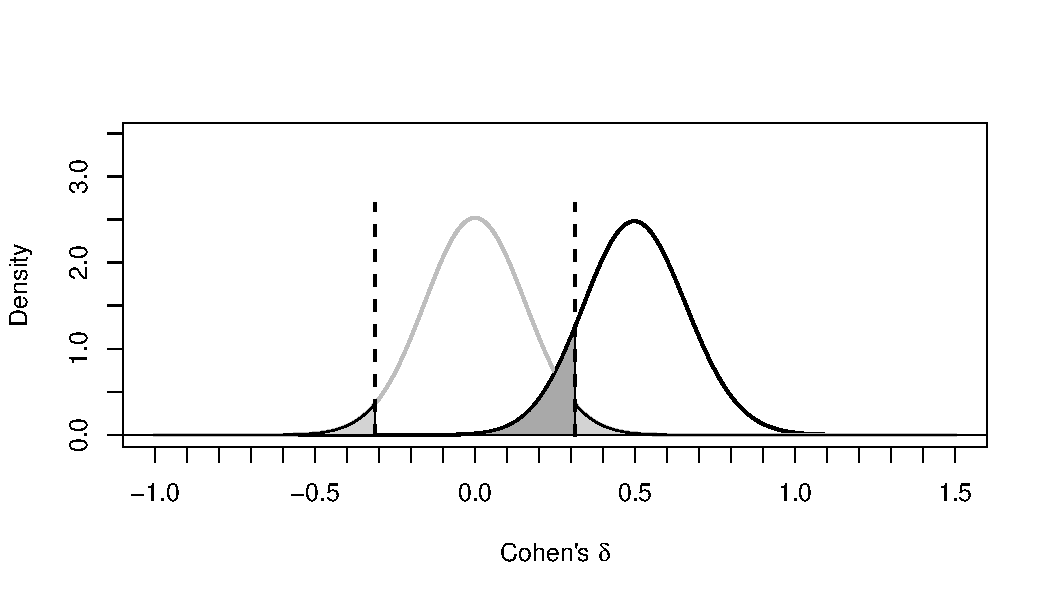
\includegraphics{0.1_Simulation_Based_Power_Analysis_For_Factorial_ANOVA_Designs_files/figure-latex/d-plot-1.pdf}
\caption{\label{fig:d-plot}Distribution of Cohen's d under the null-hypothesis (grey curve) and alternative hypothesis assuming d = 0.5 (black curve) given n = 80.}
\end{figure}

\begin{figure}
\centering
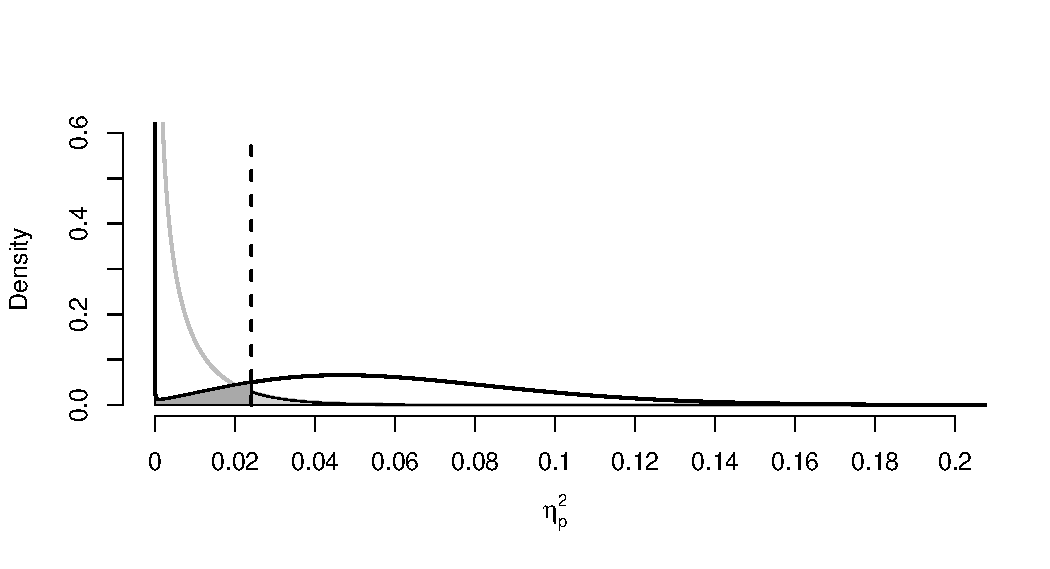
\includegraphics{0.1_Simulation_Based_Power_Analysis_For_Factorial_ANOVA_Designs_files/figure-latex/eta-plot-1.pdf}
\caption{\label{fig:eta-plot}Distribution of eta-squared under the null-hypothesis (grey curve) and alternative hypothesis assuming partial eta-squared = 0.0588 (black curve) given n = 80.}
\end{figure}

A test result is statistically significant when the \emph{p}-value is smaller than the alpha level, or when the test statistical (e.g., a \emph{F}-value) is larger than a critical value.
For a given sample size we can also calculate a critical \emph{effect size}, and a result is statistically significant if the observed effect size is more extreme than the critical effect size.
Given the sample size of 80 participants per group, observed effects are statistically significant when they are larger than d = 0.31 in a \emph{t}-test, or \(\eta_p^2\) = 0.02 for the \emph{F}-test.
The goal of an a-priori power analysis is to design a study with a desired probability of observing a significant effect.
To calculate the sample size required to reach a desired statistical power one has to specify the alternative hypothesis, the sample size, and the alpha level.
Based on \(\lambda\) (the noncentrality parameter, which together with the degrees of freedom specifies the shape of the expected effect size distribution under a specified alternative hypothesis, illustrated by the black curves in Figure \ref{fig:d-plot} and \ref{fig:eta-plot}) we can calculate the area under the curve that is more extreme than the critical effect size (i.e., Figure \ref{fig:eta-plot} to the right of the critical effect size).
Under the alternative hypothesis that the true effect size is d = 0.5 or \(\eta_p^2\) = 0.0588, data are collected from 80 participants in each condition, and an alpha of 0.05 is used, in the long run 88.16\% of the tests will yield a statistically significant result.

\begin{tcolorbox}[colback=black!5!white,colframe=white!5!black,title=Box 1. Formula for effect sizes for ANOVA designs]
For two independent groups, the \textit{t}-statistic can easily be translated to the \textit{F}-statistic $F = t^2$.
Cohen's d, a standardized effect size, is calculated by dividing the difference between means by the standard deviation, or 
\begin{equation}
d = \frac{m_1-m_2}{\sigma}.
\end{equation}
The generalization of Cohen's d to more than two groups is Cohen's $f$, which is the standard deviation of the means divided by the standard deviation (Cohen, 1988), or: 
\begin{equation}
f = \frac{\sigma _{ m }}{\sigma}
\end{equation}
where for equal sample sizes,
\begin{equation}
\sigma _{ m } = \sqrt { \frac { \sum_ { i = 1 } ^ { k } ( m _ { i } - m ) ^ { 2 } } { k } }.
\end{equation}
For two groups Cohen's $f$ is half as large as Cohen's d, or $f = \frac{1}{2}d$.
Partial eta-squared, which is often used as input in power analysis software, can be converted into Cohen's $f$:
\begin{equation}
f = \sqrt{\frac{\eta_p^2}{1-\eta_p^2}} \label{eq:eta-to-f}
\end{equation}
and Cohen's $f$ can be converted into partial eta-squared:
\begin{equation}
\eta_p^2 = \sqrt{\frac{f^2}{f^2+1}} \label{eq:f-to-eta}
\end{equation}
Power calculations rely on the noncentrality parameter (lambda, ($\lambda$).) 
In a between-participants one-way ANOVA lambda is calculated as:
\begin{equation}
\lambda = f^2 \times N \label{eq:lambda}
\end{equation}
where f is Cohen's $f$ and N is the total sample size. 
\end{tcolorbox}

\hypertarget{simulating-statistical-power-for-different-factorial-designs}{%
\section{Simulating Statistical Power for Different Factorial Designs}\label{simulating-statistical-power-for-different-factorial-designs}}

Superpower can be used in R or in an online Shiny app.
The code underlying the Superpower R package and the Shiny app generates data for each condition in the design and performs an ANOVA and \emph{t}-tests for all comparisons between conditions.
The ANOVA\_exact function simulates an \enquote{exact} dataset that has exactly the desired statistical properties, and computes power directly from the test results on this perfect dataset.
The ANOVA\_power function simulates datasets repeatedly based on the specified parameters and calculates the percentage of statistically significant results.
The simulation can be performed based on any design specified using the ANOVA\_design function, the result of which is stored and passed on to either of the two functions to compute power.
Users specify the design based on the number of levels for each factor (e.g., 2) and whether the factor is manipulated within or between participants (be entering a \enquote{w} or a \enquote{b}).
Superpower can handle up to three factors (seperated by \enquote{*}).
A 2b design means a single factor with two groups manipulated between participants, whereas a 2b*2w design is a 2 x 2 mixed ANOVA where the first factor is manipulated between, and the second within participants.
Users also specify the sample size per group (n), the predicted pattern of means across all conditions, the expected standard deviation, and the correlation between variables (for within designs).
To make it easier to interpret the output users can specify factor names and names for each factor level (e.g., \enquote{condition, cheerful, sad}).
Detailed examples for a wide range of designs are available in an online manual at \url{http://arcaldwell49.github.io/SuperpowerBook}.

An example of the R code is:

\begin{Shaded}
\begin{Highlighting}[]
\NormalTok{design_result <-}\StringTok{ }\KeywordTok{ANOVA_design}\NormalTok{(}
  \DataTypeTok{design =} \StringTok{"2b"}\NormalTok{, }
  \DataTypeTok{n =} \DecValTok{80}\NormalTok{,}
  \DataTypeTok{mu =} \KeywordTok{c}\NormalTok{(}\DecValTok{1}\NormalTok{, }\DecValTok{0}\NormalTok{), }
  \DataTypeTok{sd =} \DecValTok{2}\NormalTok{,}
  \DataTypeTok{labelnames =} \KeywordTok{c}\NormalTok{(}\StringTok{"condition"}\NormalTok{, }\StringTok{"cheerful"}\NormalTok{, }\StringTok{"sad"}\NormalTok{))}
\end{Highlighting}
\end{Shaded}

An example of the input in the Shiny app is:

\begin{figure}
\centering
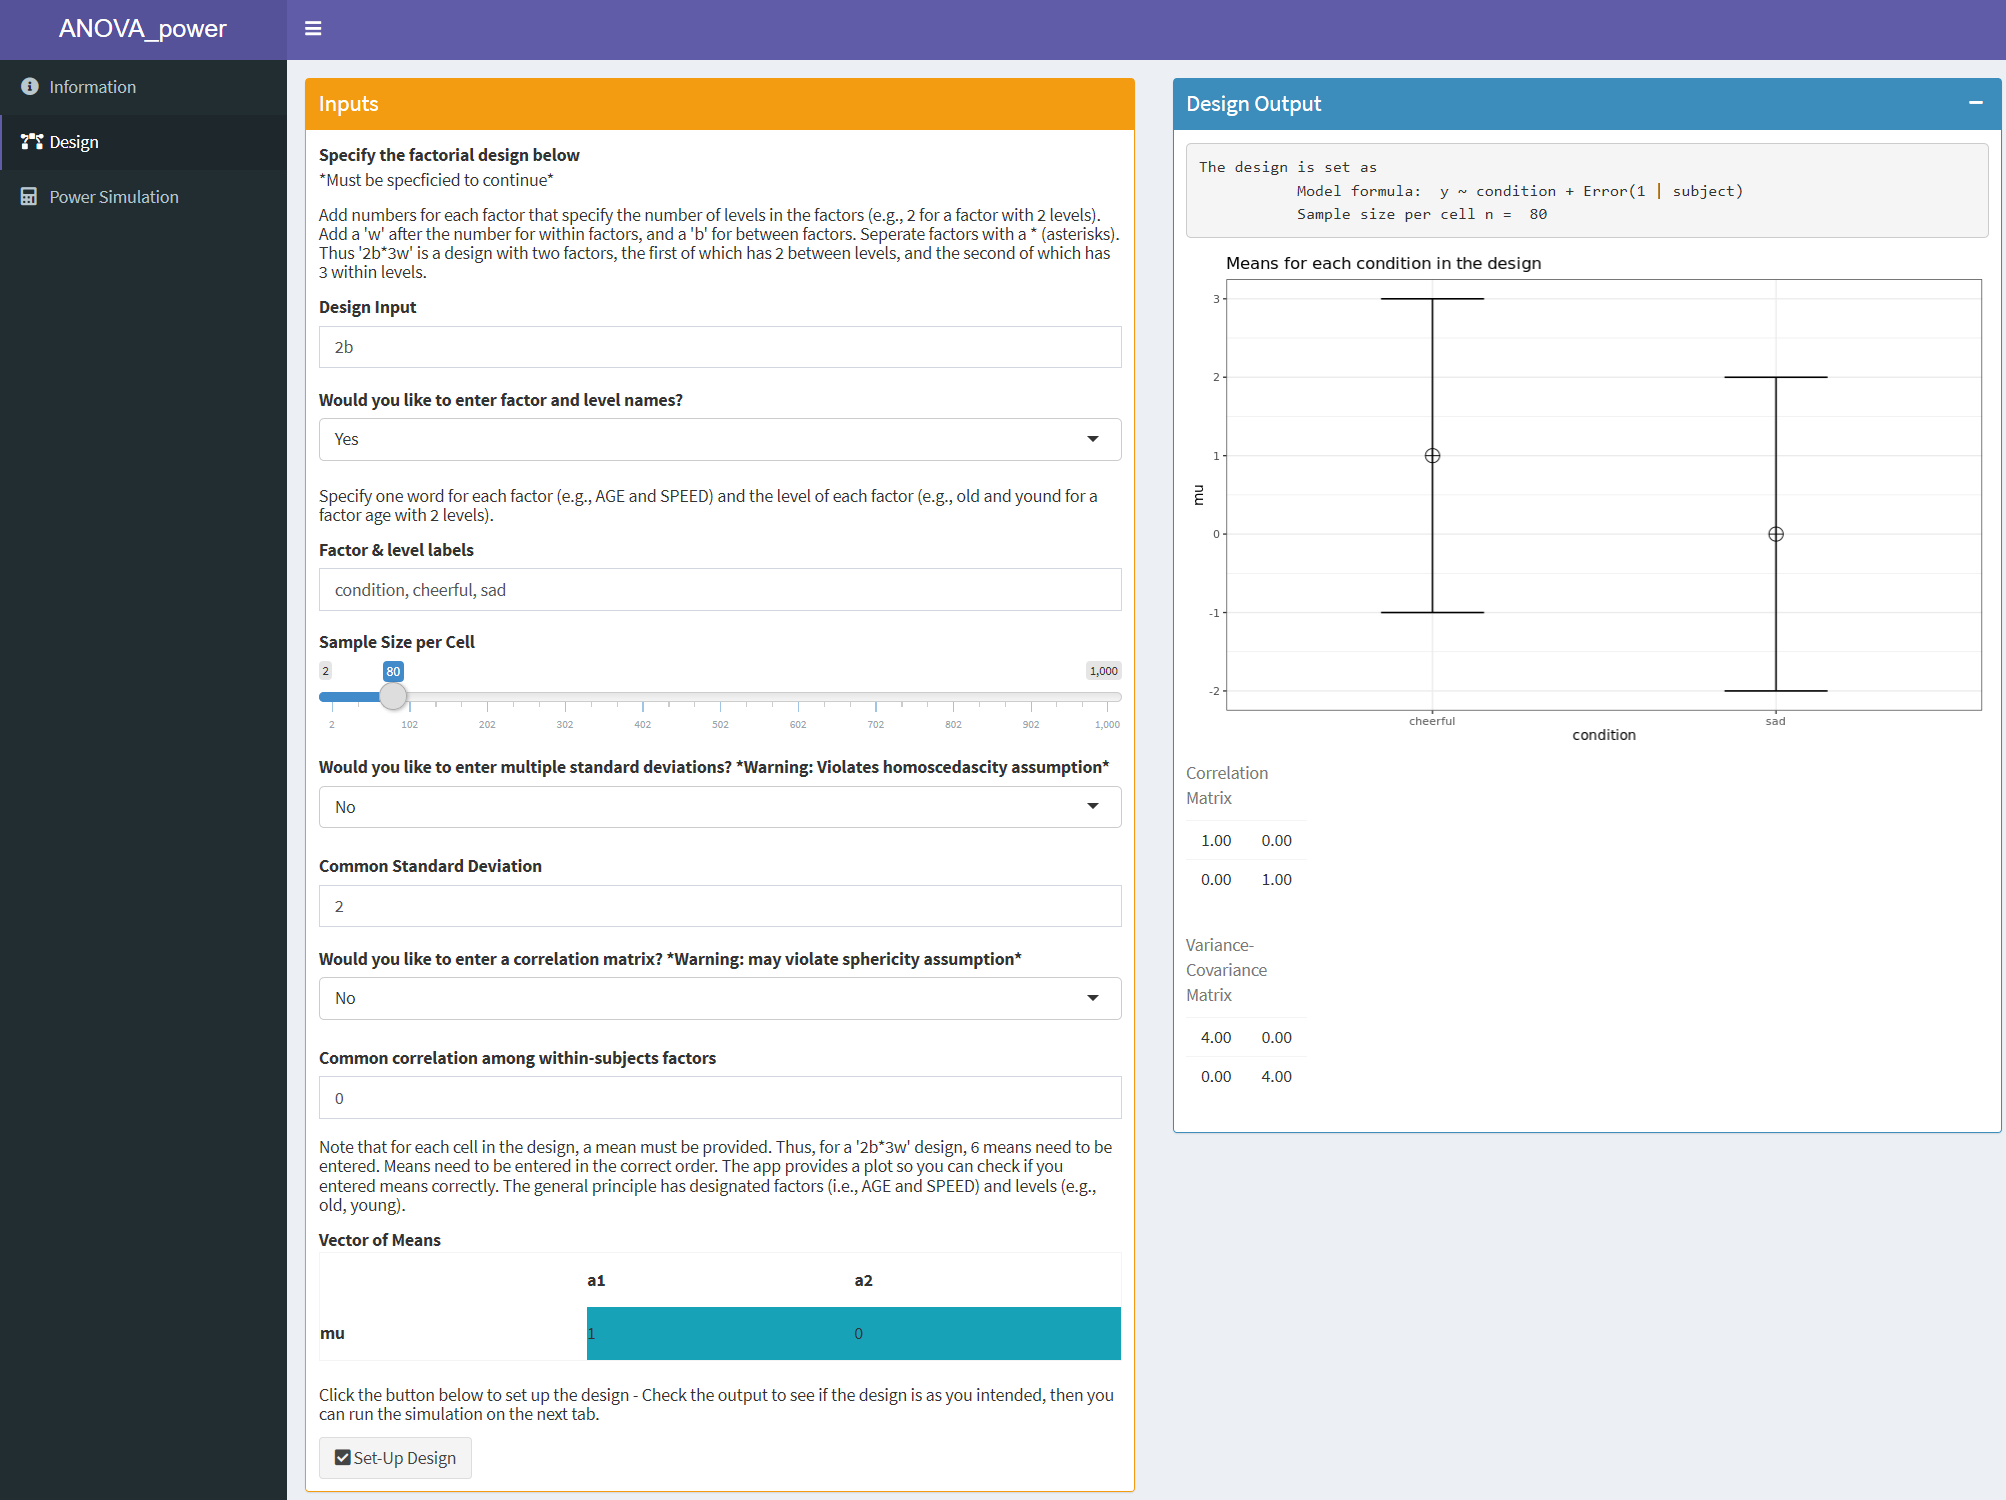
\includegraphics{screenshots/anova_power.png}
\caption{Screenshot of ANOVA\_power Shiny app.}
\end{figure}

For a visual confirmation of the input a figure is created that displays the means and standard deviation (see the right side of Figure 3).
After the design has been specified there are two ways to calculate the statistical power of an ANOVA through simulations.
The first is to repeatedly simulate datasets and compute the percentage of statistically significant results. This is completed with the ANOVA\_power function which performs a Monte Carlo simulation.

\begin{Shaded}
\begin{Highlighting}[]
\NormalTok{power_result_monte <-}\StringTok{ }\KeywordTok{ANOVA_power}\NormalTok{(design_result, }\DataTypeTok{nsims =} \DecValTok{100000}\NormalTok{)}
\end{Highlighting}
\end{Shaded}

The second is to simulate a dataset that has \emph{exactly} the desired properties, perform an ANOVA, and use the ANOVA results to compute the statistical power. This is completed with the \texttt{ANOVA\_exact} function which performs a \enquote{exact} simulation.

\begin{Shaded}
\begin{Highlighting}[]
\NormalTok{power_result_exact <-}\StringTok{ }\KeywordTok{ANOVA_exact}\NormalTok{(design_result)}
\end{Highlighting}
\end{Shaded}

The first approach is a bit more flexible (e.g., it allows for sequential corrections for multiple comparisons such as the Holm procedure), but the second approach is much faster (and generally recommended).
There is often uncertainty about the values that need to be entered a-priori power analysis because the true (population-level) pattern of the data are unknown.
It makes sense to examine power across a range of assumptions, from more optimistic scenarios, to more conservative estimates.
In many cases researchers should consider collecting a sample size that guarantees sufficient power for the smallest effect size of interest, instead of the effect size they expect (for examples, see Lakens, Scheel, and Isager (2018)).
This approach ensures the study can be informative, even when there is uncertainty about the true effect size.
If ANOVA\_power is used the results from the simulation will vary each time the simulation is performed (unless a seed is specified, e.g., `set.seed = 2019').
A user should specify the number of simulations (the more simulations, the more accurate the results are,, but the longer the simulation takes), the alpha level for the tests, and any adjustments for multiple comparisons that are required.
The output from ANOVA\_exact and ANOVA\_power are similar, and provides the statistical power for the ANOVA and all simple comparisons between conditions.

\begin{verbatim}
Power and Effect sizes for ANOVA tests
                    power effect_size
anova_condition    88.191     0.06425

Power and Effect sizes for pairwise comparisons (t-tests)
                                       power effect_size
p_condition_cheerful_condition_sad    88.191     -0.5017
\end{verbatim}

The same results are returned in the onine Shiny app, but here users can also choose a \enquote{download PDF report} option to receive the results as a PDF file that can be saved to be included as documentation for sample size requirements (e.g., preregistrations, Registered Reports, or grant applications).

\begin{figure}
\centering
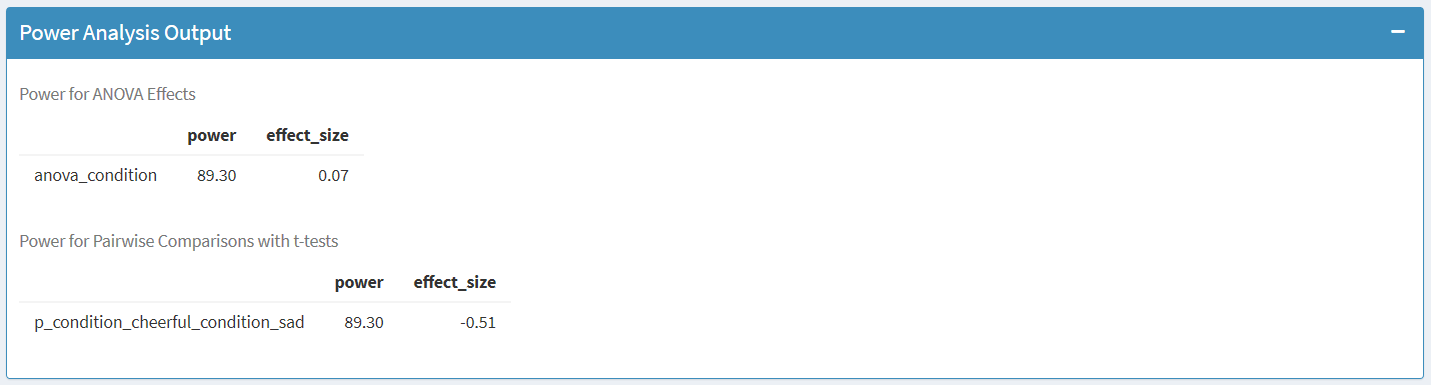
\includegraphics{screenshots/anova_power_result.png}
\caption{Screenshot of the results of the power analysis in the ANOVA\_power Shiny app.}
\end{figure}

From these results we see that when 100.000 simulations are performed for our two group between subjects design with means of 1 and 0, a standard deviation of 2, and 80 participants in each group, with a seed set to 2019 (these settings will be used for all simulation results reported in this manuscript), the statistical power (based on the percentage of \emph{p} \textless{} \(\alpha\) results) is 88.19\% and the average \(\eta_p^2\) is 0.06.
The simulation also provides the results for the individual comparisons based on \emph{t}-tests.
Since there are only two groups in this example, the statistical power for the individual comparison is identical to the ANOVA, but the expected effect size is given in Cohen's d: -0.50.

Now that the basic idea behind power analyses in Superpower is illustrated, we can use it to explore how changes to the experimental design influence power, and answer some of the questions our hypothetical researcher is confronted with when designing a follow-up study.
We will first examine what happens if we add a third, neutral, condition to the design.
Let's assume a researcher expects the mean enjoyment rating for the neutral voice condition to fall either perfectly between the cheerful and sad conditions, or to be equal to the cheerful condition.
The researcher wonders if simply collecting 80 additional participants in the neutral condition is enough for a one-way ANOVA to have sufficient power.
The R code to specify this design is:

\begin{Shaded}
\begin{Highlighting}[]
\NormalTok{design_result_}\DecValTok{1}\NormalTok{ <-}\StringTok{ }\KeywordTok{ANOVA_design}\NormalTok{(}
  \DataTypeTok{design =} \StringTok{"3b"}\NormalTok{, }
  \DataTypeTok{n =} \DecValTok{80}\NormalTok{, }
  \DataTypeTok{mu =} \KeywordTok{c}\NormalTok{(}\DecValTok{1}\NormalTok{, }\FloatTok{0.5}\NormalTok{, }\DecValTok{0}\NormalTok{),}
  \DataTypeTok{sd =} \DecValTok{2}\NormalTok{, }
  \DataTypeTok{labelnames =} \KeywordTok{c}\NormalTok{(}\StringTok{"condition"}\NormalTok{, }\StringTok{"cheerful"}\NormalTok{, }\StringTok{"neutral"}\NormalTok{, }\StringTok{"sad"}\NormalTok{))}
\end{Highlighting}
\end{Shaded}

The design now has 3 between-participant conditions, and we can explore what happens if we would collect 80 participants in each condition.

If we assume the mean falls exactly between between the cheerful and sad conditions, the simulations show the statistical power for a 3-groups one-way ANOVA \emph{F}-test is reduced to 81.14 \%, and the effect size (partial eta-squared) is 0.05.
If we assume the mean is equal to the cheerful condition, the power increases to 91.03\%.
Compared to the two group design (where the power was 88.19\%), three things have changed.
First, the numerator degrees of freedom has increased because an additional group is added to the design, which makes the non-central \emph{F}-distribution more similar to the central \emph{F}-distribution, which reduces the statistical power.
Second, the total sample size is 50\% larger after adding 80 participants in the third condition, which increases the statistical power of the ANOVA.
Third, the effect size, Cohen's \(f\), has decreased from 0.25 to either 0.20 or 0.24, which reduces the statistical power.
The most important take-home message is that changing an experimental design can have several opposing effects on the power of a study, depending of the pattern of means.
The exact effect of these three changes on the statistical power is difficult to anticipate from one design to the next.
This highlights the importance of performing an a-priori power analysis based on a specific pattern of means that your theory or hypotheses predict.

Although an initial goal when might be to test the \emph{omnibus null hypothesis} (i.e., ANOVA), which answers the question whether there are \emph{any} differences between group means, we often want to know which \emph{specific} conditions differ from each other.
Thus, an ANOVA is often followed up by individual comparisons (whether \emph{planned} or \emph{post-hoc}).
Superpower automatically provides the statistical power for all individual comparisons that can be performed.
By default, the power and effect size estimates are based on simple \emph{t}-tests.
It is also possible to combine variance estimates from all conditions and calculate the estimated marginal means (Lenth, 2019) when performing individual comparisons by setting \texttt{emm\ =\ TRUE} within the ANOVA\_power or ANOVA\_exact functions, or checking this option in the Shiny app.
This approach is often has greater statistical power (Maxwell, Delaney, \& Kelley, 2017), depending on whether the assumption of equal variances (also known as the homogeneity assumption) is met, which may not be warranted in psychological research (Delacre, Lakens, Mora, \& Leys, 2018).
The degree to which violations of the homogeneity assumption affect Type 1 error rates can be estimated with the ANOVA\_power function (see Assumptions section below).
Power analysis for individual comparisons is relatively straightforward and can easily be done in all power analysis software, but providing power for all individual comparisons alongside the ANOVA result by default hopefully nudges researchers to take into account the power for follow-up tests.

When performing multiple individual comparisons, we need to choose the alpha level and ensure the Type 1 error rate is not inflated.
By adjusting for multiple comparisons we ensure that we do not conclude there is an effect in \emph{any} of the individual tests more often than the desired Type 1 error rate.
Several techniques to control error rates exist, of which the best known is the Bonferroni correction.
The Holm procedure is slightly more powerful than the Bonferroni correction, without requiring additional assumptions (for other approaches, see Bretz, Hothorn, \& Westfall, 2011).
Power analyses using a manually calculated Bonferoni correction can be performed with the ANOVA\_exact function by specifying the adjusted alpha level, but the sequential Holm approach can only be performed in the ANOVA\_power simulation approach.
Because the adjustment for multiple comparisons lowers the alpha level, it also lowers the statistical power.
For the paired comparisons we see we have approximately 80\% power for differences of 0.5 after controlling for multiple comparisons with the Holm procedure (compared to 88\% power without correcting for multiple comparisons).
As the number of possible paired comparisons increases, the alpha level is reduced, and power becomes lower, all else equal.
These power analyses reveal the cost (in terms of the statistical power) of exploring across all possible paired comparisons while controlling error rates.
To maintain an adequate level of power after lowering the alpha level to control the Type 1 error rate after multiple comparisons the sample size should be increased.
In a one-way ANOVA multiple comparisons are only an issue for the follow-up comparison, but in a 2x2x2 design, an ANOVA will give the test results for three main effects, three two-way interactions, and one three-way interaction.
Because seven statistical tests are performed, the probability of making at least one Type 1 error in a single exploratory 2x2x2 ANOVA is \(1-(0.95)^7\) = 30\%.
It is therefore important to control error rates in exploratory ANOVA's (Cramer et al., 2016).
If a researcher is only interested in specific tests it is advisable to preregister and test only these comparisons instead of correcting the alpha level for all possible comparisons (Haans, 2018).

\hypertarget{power-for-within-subject-designs}{%
\section{Power for Within-Subject Designs}\label{power-for-within-subject-designs}}

What happens if we would perform the second study as a within-participants design?
Instead of collecting three groups of participants, we only collect one group, and let this group evaluate the cheerful, neutral, and sad voice assistants.
If we want to examine the power for a within design we need to enter our best estimate for the true population value of the correlation between dependent measurements.
Ideally this value is determined based on previous studies, and when there is substantial uncertainty about the true population value it often makes sense to explore a range of plausible correlations.
Let's assume our best estimate of the correlation between enjoyment ratings in a within-subject design is \emph{r} = 0.5.
The ANOVA\_design function below specifies this design.
Note the design has changed from \texttt{3b} (a one factor between design with three levels) to \texttt{3w} (a one factor within design with three levels) and the correlation parameter \texttt{r\ =\ 0.5} is added, which specifies the expected correlation between dependent variables in the population.

\begin{Shaded}
\begin{Highlighting}[]
\NormalTok{design_result_within_}\DecValTok{1}\NormalTok{ <-}\StringTok{ }\KeywordTok{ANOVA_design}\NormalTok{(}
  \DataTypeTok{design =} \StringTok{"3w"}\NormalTok{,}
  \DataTypeTok{n =} \DecValTok{80}\NormalTok{,}
  \DataTypeTok{mu =} \KeywordTok{c}\NormalTok{(}\DecValTok{1}\NormalTok{, }\FloatTok{0.5}\NormalTok{, }\DecValTok{0}\NormalTok{),}
  \DataTypeTok{sd =} \DecValTok{2}\NormalTok{,}
  \DataTypeTok{r =} \FloatTok{0.5}\NormalTok{,}
  \DataTypeTok{labelnames =} \KeywordTok{c}\NormalTok{(}\StringTok{"condition"}\NormalTok{, }\StringTok{"cheerful"}\NormalTok{, }\StringTok{"neutral"}\NormalTok{, }\StringTok{"sad"}\NormalTok{)}
\NormalTok{)}
\end{Highlighting}
\end{Shaded}

A rough but useful approximation of the sample size needed in a within-subject design (\(N_W\)), relative to the sample needed in between-design (\(N_B\)), is (from Maxwell \& Delaney, 2004, p.~562, formula 47):
\begin{equation}
N_{W}=\frac{N_{B}(1-\rho)}{a} \label{eq:within-n}
\end{equation}
Here \(a\) is the number of within-participant levels, \(\rho\) is the correlation between measurements in the population.
From this formula we see that switching from a between to a within design reduces the required sample size simply because each participant contributes data to each condition, even if the correlation between measurements is 0.
In our example a within design would require three times as few participants as a between subjects design with three conditions.
If the correlation between dependent variables is positive, the standard deviation of the difference scores is smaller in a within design than in a between design.
Because the standardized effect size is the mean difference divided by the standard deviation of the difference scores, a positive correlation increases the standardized mean difference in a within-subject design, which increases the statistical power.

We can perform the simulation-based power analysis with the \texttt{ANOVA\_power} or \texttt{ANOVA\_exact} functions.

\begin{Shaded}
\begin{Highlighting}[]
\NormalTok{power_result_within_}\DecValTok{1}\NormalTok{ <-}\StringTok{ }\KeywordTok{ANOVA_power}\NormalTok{(design_result_within_}\DecValTok{1}\NormalTok{, }
                                     \DataTypeTok{nsims =} \DecValTok{100000}\NormalTok{)}

\NormalTok{exact_result_within_}\DecValTok{1}\NormalTok{ <-}\StringTok{ }\KeywordTok{ANOVA_exact}\NormalTok{(design_result_within_}\DecValTok{1}\NormalTok{)}
\end{Highlighting}
\end{Shaded}

Revisiting our between-participant design, power was 81.14\% when the enjoyment scores were uncorrelated.
The power for a repeated-measures ANOVA based on these values, where ratings for the three conditions are collected from 80 participants, is 98.38\%.
Because of the positive correlation between dependent variables, the effect size \(\eta_p^2\) is much larger for the within-subject design (\(\eta_p^2\) = 0.12) than for the 3 group between participants design (\(\eta_p^2\) = 0.05), and a researcher might deside to collect somewhat less participants, while staying having a sufficiently low Type 2 error rate.
As explained in Box 2 G*Power by default uses a different calculation for \(\eta_p^2\) which does not depend on the correlation.
This default often leads to errors for power analyses that include within-subject factors when researchers perform a power analysis on an effect size reported in the published literature.
The Superpower package allows researchers to enter a correlation matrix that specifies the expected population correlation for each pair of measurements (i.e., correlation matrix), instead of entering a single correlation as in the example above.

\textbackslash{}begin\{tcolorbox\}{[}colback=black!5!white,colframe=white!5!black,title=Box 2. Formula for effect sizes for within designs{]}
The effect size in a within-design is referred to as Cohen's \(d_z\) (because it is the effect size of the difference score between \textit{x} and \textit{y}, yielding \textbackslash{}textit\{\{z\}). The relation is:
\begin{equation}
\sigma_{z}=\sigma\sqrt{2(1-\rho)}
\end{equation}
Cohen's \(d_z\) is used in power analyses for dependent \(t\)-tests, but there is no equivalent Cohen's \(f_z\) for a within-participant ANOVA, and Cohen's \(f\) is identical for within and between designs.
Instead, the value for lambda (\(\lambda\)) is adjusted based on the correlation.
For a one-way within-participant design lambda is identical to Equation \eqref{eq:lambda}, multiplied by \textit{u}, a correction for within-subject designs, calculated as:
\begin{equation}
u = \frac{k}{1-\rho}
\end{equation}
where \(k\) is the number of levels of the within-participant factor, and \(\rho\) is the correlation between dependent variables.
Equations 4 and 5 no longer hold when measurements are correlated.
The default settings in G*Power expects an f or \(\eta_p^2\) that does not incorporate the correlation, while the correlation is incorporated in the output of software packages such as SPSS.
One can enter the \(\eta_p^2\) from SPSS output in G*Power after checking the \enquote{as in SPSS} checkbox in the options window, but forgetting this is a common mistake in power analyses for within designs in G*Power.
For a one-way within-subject design, Cohen's \(f\) can be converted into the Cohen's \(f\) SPSS uses through:
\begin{equation}
f^2_{SPSS} = f^2 \times \frac{k}{k-1} \times \frac{n}{n-1} \times \frac{1}{1-\rho}
\end{equation}
and subsequently tranformed to \(\eta_p^2\) through Equation 5.
\textbackslash{}end\{tcolorbox\}

\hypertarget{power-for-interactions}{%
\section{Power for Interactions}\label{power-for-interactions}}

So far we have explored power analyses for one factor designs.
Superpower can easily provide statistical power for designs with up to three factors of up to 999 levels (e.g., a 4b*2w*2w would specify a mixed design with two within factors which 2 levels, and one between factor with 4 levels).
Let's assume the researcher plans to perform a follow-up experiment where in addition to making the voice sound cheerful or sad, a second factor is introduced by making the voice sound more robotic compared to the default human-like voice.
Different patterns of results could be expected in this 2 by 2 design that lead to interactions.
Either no effect is observed for robotic voices, or the opposite effect is observed for robotic voices (we enjoy a sad robotic voice more than a cheerful one, a \enquote{Marvin-the-Depressed-Robot Effect}).
We specify the pattern of means as \texttt{(1,\ 0,\ 0,\ 0)} for the ordinal interactions, or as \texttt{(1,\ 0,\ 0,\ 1)} for the cross-over (or disordinal) interaction, as illustrated below (see Figure \ref{fig:mean-plot} for the expected pattern of means).

\begin{Shaded}
\begin{Highlighting}[]
\NormalTok{design_result_cross_}\DecValTok{80}\NormalTok{ <-}\StringTok{ }\KeywordTok{ANOVA_design}\NormalTok{(}
  \DataTypeTok{design =} \StringTok{"2b*2b"}\NormalTok{,}
  \DataTypeTok{n =} \DecValTok{80}\NormalTok{,}
  \DataTypeTok{mu =} \KeywordTok{c}\NormalTok{(}\DecValTok{1}\NormalTok{, }\DecValTok{0}\NormalTok{, }\DecValTok{0}\NormalTok{, }\DecValTok{1}\NormalTok{),}
  \DataTypeTok{sd =} \DecValTok{2}\NormalTok{,}
  \DataTypeTok{labelnames =} \KeywordTok{c}\NormalTok{(}\StringTok{"condition"}\NormalTok{, }\StringTok{"cheerful"}\NormalTok{, }\StringTok{"sad"}\NormalTok{, }
                 \StringTok{"voice"}\NormalTok{, }\StringTok{"human"}\NormalTok{, }\StringTok{"robot"}\NormalTok{)}
\NormalTok{)}
\end{Highlighting}
\end{Shaded}

\begin{figure}
\centering
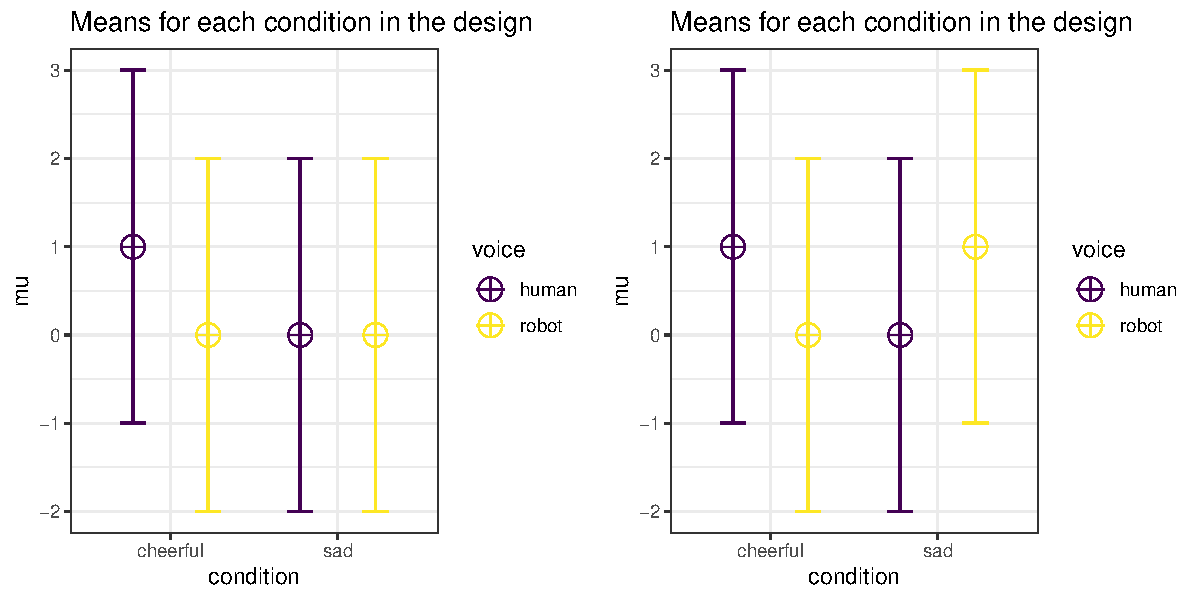
\includegraphics{0.1_Simulation_Based_Power_Analysis_For_Factorial_ANOVA_Designs_files/figure-latex/mean-plot-1.pdf}
\caption{\label{fig:mean-plot}Vizualization for the expected means and standard deviations for an ordinal (left) and crossover (right) interaction. Error bars represent one standard deviation.}
\end{figure}

\begin{tcolorbox}[colback=black!5!white,colframe=white!5!black,title=Box 3. Calculating effect sizes for interactions]
Mathematically the interaction effect is computed as the cell mean minus the sum of the grand mean, the marginal mean in each condition of one factor minus the grand mean, and the marginal mean in each condition for the other factor minus grand mean (see Maxwell et al., 2017). For example, for the cheerful human-like voice condition in the cross-over interaction this is 1 (the value in the cell) - (0.5 [the grand mean] + 0 [the marginal mean of cheerful voices minus the grand mean of 0.5] + 0 [the marginal mean of human-like voices minus the grand mean of 0.5]). 
Thus, 1 - (0.5 + 0 + 0) = 0.5.
Completing this for all four cells for the cross-over interaction gives the values 0.5, -0.5, -0.5, 0.5.
Cohen's $f$ is then $f = \frac { \sqrt { \frac { 0.5^2 +-0.5^2 + -0.5^2 + -0.5^2 } { 4 } }}{ 2 } = 0.25$.
For the ordinal interaction the grand mean is (1+0+0+0)/4, or 0.25.
Completing the calculation for all four cells for the ordinal interaction gives the values 0.25, -0.25, -0.25, 0.25, and a Cohen's $f$ of 0.125. 
We see the effect size of the cross-over interaction is twice as large as the effect size of the ordinal interaction. 
Had we predicted a pattern of means of 2, 0, 0, 0, then the effect size for the ordinal interation would have been f = 0.25. 
The take-home message is that a 'medium' effect size (f = 0.25) translates into a much more extreme pattern of means in an ordinal interaction than in a disordinal (crossover) interaction, or in a 2x2x2 interaction compared to a 2x2 interaction (see also Perugini et al. (2018)).
It might therefore be more intuitive to perform a power analysis based on the expected pattern of means, than to perform a power analyses based on Cohen's $f$ or $\eta_p^2$.
\end{tcolorbox}

Simulations (using either the ANOVA\_power or ANOVA\_exact functions) show we have 99.38\% power for the cross-over interaction when we collect 80 participants per condition, and 60.62\% power for the ordinal interaction.
For comparison, the power for the simple effect corresponding to one-way ANOVA example we started with is 88.16\%.
The cross-over interaction has much higher statistical power than the ordinal interaction because the effect size is twice as large, as explained in Box 3.
The cross-over interaction also has more statistical power than the simple comparison, even though the effect size is identical (Cohen's \(f\) = 0.25) because the sample size has doubled.
The interaction effect can be contrast coded as 1, -1, -1, 1, and thus tests the scores of 160 participants in the cheerful human and sad robot conditions against the scores of 160 participants in the cheerful robot and sad human conditions.
The key insight here is that not the sample size per condition, but the pooled sample size across conditions compared in a contrast that determines the power for the main effects and the interaction (cf.~J. Westfall, 2015b).

Superpower also allows users to plot the statistical power across a range of sample sizes for the ANOVA\_exact function (when using the ANOVA\_power function, users will need to steadily increase or decrease the sample size in their simulations).
This allows us to take a look at the statistical power the design has across a range of effects size.
The code below plots the power from 10 participants per condition to 100 participants per condition for the ordinal interaction (see Figure \ref{fig:power-plot}).

\begin{Shaded}
\begin{Highlighting}[]
\NormalTok{plot_data <-}\StringTok{ }\KeywordTok{plot_power}\NormalTok{(design_result_cross_}\DecValTok{80}\NormalTok{, }
                        \DataTypeTok{min_n =} \DecValTok{10}\NormalTok{, }\DataTypeTok{max_n =} \DecValTok{100}\NormalTok{, }
                        \DataTypeTok{plot =} \OtherTok{TRUE}\NormalTok{)}
\end{Highlighting}
\end{Shaded}

\begin{figure}
\centering
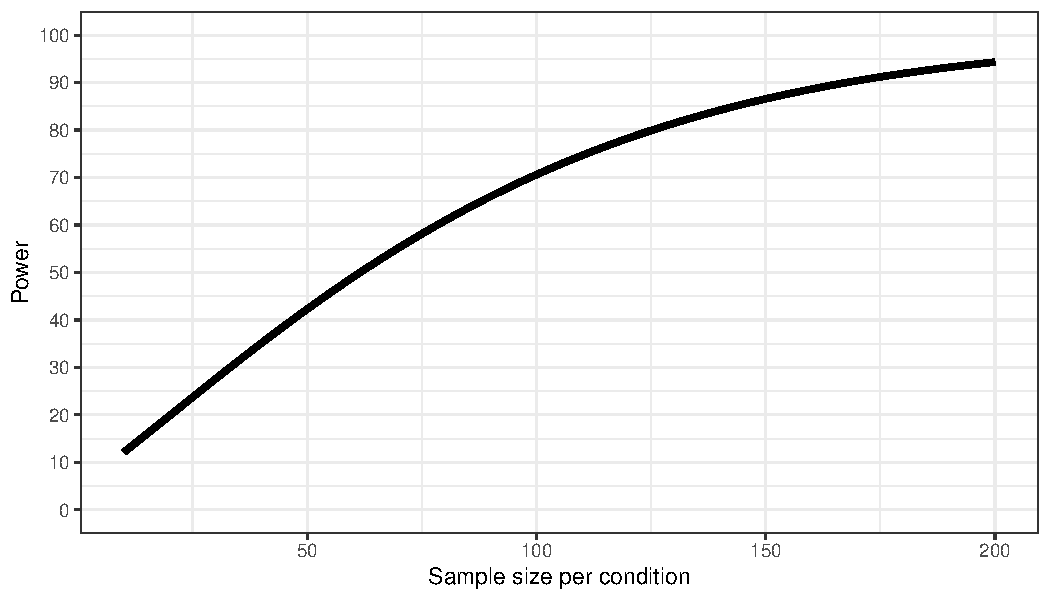
\includegraphics{0.1_Simulation_Based_Power_Analysis_For_Factorial_ANOVA_Designs_files/figure-latex/power-plot-1.pdf}
\caption{\label{fig:power-plot}Power curves across a range of sample sizes per group from n = 10 to n = 100 for the expected main effects and ordinal interaction.}
\end{figure}

The plot shows that with n = 40 per group, the ordinal interaction has the same statistical power as the one-way ANOVA example we started with, revealing that a Cohen's \(f\) = 0.25 with 40 participants in each of four conditions leads to the same power as having 80 participant in each condition.
We also see that the cross-over interaction has the same power with 20 participants per cell as the ordinal interaction with 80 participants per cell.
When the effect size is halved, the required sample size to maintain the same statistical power almost quadruples (Giner-Sorolla, 2018; Simonsohn, 2014).

\hypertarget{violation-of-assumptions}{%
\section{Violation of Assumptions}\label{violation-of-assumptions}}

So far in manuscript we have shown how simulations can be useful for power analyses for ANOVA designs where all assumptions of the statistical tests are met.
An ANOVA is quite robust against violations of the normality assumption, which means the Type 1 error rate remains close to the alpha level specified in the test. Violations of the homogeneity of variances assumption can be more impactful, especially when sample sizes are unequal between conditions.
When the equal variances assumption is violated for a one-way ANOVA Welch's \emph{F}-test is a good default.
When the sphericity assumption in within designs is violated (when the variances of the differences between all pairs are not equal) a sphericity correction can be applied (e.g., the Greenhouse-Geisser or Huynh-Feldt correction) or a Multivariate ANOVA (MANOVA) can be performed.
Alternative approaches for ANOVA designs with multiple between factors exist, such as heteroskedasticity robust standard errors.
Superpower allows researchers to perform power analyses for unequal variances (or correlations) by performing Welch' \emph{F}-test, appying sphercity corrections, or a MANOVA.

Although some recommendations have been provided to assist researchers to choose an approach to deal with violations of the homogeneity assumption (Algina \& Keselman, 1997), it is often unclear if these violations of the homogeneity assumption are consequential for a given study.
So far we have used simulations in Superpower to simulate patterns of means where there is a true effect, but we can also simulate a null effect.
Such Monte Carlo simulation studies are used in published articles to examine the Type 1 error rate under a range of assumptions and while performing different tests.
Superpower makes it easy to perform such simulations studies for the specific scenario a researcher is faced with, and can help to make a decision whether violations of assumptions are something to worry about, and whether choices to deal with violations are sufficient.

As an example, let's revisit our earlier 2x2 between subjects design.
Balanced designs (the same sample size in each condition) reduce the impact of violations of the homogeneity assumption, but let's assume that for some reason sample sizes varied between 20 and 80 per cell, and the population standard violations varied extremely across conditions (from 1 to 5).
We can use Superpower to estimate the impact of violating the homogeneity assumption by simulating a null effect (the means in all conditions are the same) and examining the Type 1 error rate.
We can specify a design with unequal sample sizes and unequal variances as illustrated in the code below.

\begin{Shaded}
\begin{Highlighting}[]
\NormalTok{design_result_violation <-}\KeywordTok{ANOVA_design}\NormalTok{(}
  \DataTypeTok{design =} \StringTok{"2b*2b"}\NormalTok{,}
  \DataTypeTok{n =} \KeywordTok{c}\NormalTok{(}\DecValTok{20}\NormalTok{, }\DecValTok{80}\NormalTok{, }\DecValTok{40}\NormalTok{, }\DecValTok{80}\NormalTok{),}
  \DataTypeTok{mu =} \KeywordTok{c}\NormalTok{(}\DecValTok{0}\NormalTok{, }\DecValTok{0}\NormalTok{, }\DecValTok{0}\NormalTok{, }\DecValTok{0}\NormalTok{),}
  \DataTypeTok{sd =} \KeywordTok{c}\NormalTok{(}\DecValTok{3}\NormalTok{, }\DecValTok{1}\NormalTok{, }\DecValTok{5}\NormalTok{, }\DecValTok{1}\NormalTok{),}
  \DataTypeTok{labelnames =} \KeywordTok{c}\NormalTok{(}\StringTok{"condition"}\NormalTok{, }\StringTok{"cheerful"}\NormalTok{, }\StringTok{"sad"}\NormalTok{, }\StringTok{"voice"}\NormalTok{, }\StringTok{"human"}\NormalTok{, }\StringTok{"robot"}\NormalTok{))}
\ErrorTok{)}
\NormalTok{power_result_violation <-}\StringTok{ }\KeywordTok{ANOVA_power}\NormalTok{(}
\NormalTok{  design_result_violation,}
  \DataTypeTok{nsims =} \DecValTok{100000}\NormalTok{)}
\end{Highlighting}
\end{Shaded}

Based on this simulation, the Type 1 error rate for the main effects and interactions for the ANOVA are approximately 15.85\%.
Under these assumptions it is clear that the Type 1 error rate is too high.
One solution would be to make sure that an experiment has equal sample sizes.
If this is achieved, the Type 1 error rate it reduced to 4.98\%, which is acceptable.

\hypertarget{conclusion}{%
\section{Conclusion}\label{conclusion}}

It is important to justify the sample size when designing a study.
Power analyses for more complex ANOVA designs have typically required programming knowledge.
The R package, guide book, and Shiny apps (see \url{https://arcaldwell49.github.io/SuperpowerBook}) that accompany this tutorial enable researchers to perform simulations for factorial experiments of up to three factors and any number of levels, making it easy to perform simulation-based power analysis without extensive programming experience.
Exploring the power for designs with specific patterns of means, standard deviations, and correlations between variables can be used to choose a design and sample size that provides the highest statistical power for future studies.
Simulation based approaches can also help to provide a better understanding of the factors that influence the statistical power for factorial ANOVA designs, or the impact of violations of assumptions on the Type 1 error rate.

\hypertarget{author-contributions}{%
\subsection{Author Contributions}\label{author-contributions}}

D. Lakens and A. R. Caldwell collaboratively developed the Superpower R package. D. Lakens wrote the initial draft, and both authors revised the manuscript. A. R. Caldwell created the Shiny apps.

\hypertarget{orcid-ids}{%
\subsection{ORCID iD's}\label{orcid-ids}}

Daniël Lakens 
\includegraphics{screenshots/orcid.png} \url{https://orcid.org/0000-0002-0247-239X}
Aaron R. Caldwell 
\includegraphics{screenshots/orcid.png} \url{https://orcid.org/0000-0002-4541-6283}

\hypertarget{acknowledgements}{%
\subsection{Acknowledgements}\label{acknowledgements}}

Many improvements to Superpower are based on feedback from Lisa DeBruine and the sim\_design function in her \enquote{faux} R package. The ANOVA\_exact function was inspired by Chris Aberson's pwr2ppl package. We are grateful to Jonathon Love for proposing the name \enquote{Superpower} and the development of a jamovi module.

\hypertarget{declaration-of-conflicting-interests}{%
\subsection{Declaration of Conflicting Interests}\label{declaration-of-conflicting-interests}}

The opinions or assertions contained herein are the private views of the author(s) and are not to be construed as official or reflecting the views of the Army or the Department of Defense. Any citations of commercial organizations and trade names in this report do not constitute an official Department of the Army endorsement of approval of the products or services of these organizations. Approved for public release; distribution is unlimited. The author(s) declared that there were no conflicts of interest with respect to the authorship or the publication of this article.

\hypertarget{funding}{%
\subsection{Funding}\label{funding}}

This work was funded by VIDI Grant 452-17-013 from the Netherlands Organisation for Scientific Research.

\hypertarget{open-practices}{%
\subsection{Open Practices}\label{open-practices}}

The code to reproduce the analyses reported in this article has been made publicly available via the Open Science Framework and can be accessed at \url{https://osf.io/pn8mc/}.

\hypertarget{references}{%
\subsection{References}\label{references}}

\setlength{\parindent}{-0.5in}
\setlength{\leftskip}{0.5in}

\hypertarget{refs}{}
\leavevmode\hypertarget{ref-aberson_applied_2019}{}%
Aberson, C. L. (2019). \emph{Applied Power Analysis for the Behavioral Sciences} (2nd ed.). New York: Routledge.

\leavevmode\hypertarget{ref-algina_detecting_1997}{}%
Algina, J., \& Keselman, H. J. (1997). Detecting repeated measures effects with univariate and multivariate statistics. \emph{Psychological Methods}, \emph{2}(2), 208--218. doi:\href{https://doi.org/10.1037/1082-989X.2.2.208}{10.1037/1082-989X.2.2.208}

\leavevmode\hypertarget{ref-bretz_multiple_2011}{}%
Bretz, F., Hothorn, T., \& Westfall, P. H. (2011). \emph{Multiple comparisons using R}. Boca Raton, FL: CRC Press.

\leavevmode\hypertarget{ref-brysbaert_how_2019}{}%
Brysbaert, M. (2019). How many participants do we have to include in properly powered experiments? A tutorial of power analysis with some simple guidelines. \emph{Journal of Cognition}.

\leavevmode\hypertarget{ref-Campbell2012MorePower6F}{}%
Campbell, J., \& Thompson, V. A. (2012). MorePower 6.0 for anova with relational confidence intervals and bayesian analysis. \emph{Behavior Research Methods}, \emph{44}, 1255--1265. Retrieved from \url{https://doi.org/10.3758/s13428-012-0186-0}

\leavevmode\hypertarget{ref-cohen_statistical_1988}{}%
Cohen, J. (1988). \emph{Statistical power analysis for the behavioral sciences} (2nd ed.). Hillsdale, N.J: L. Erlbaum Associates.

\leavevmode\hypertarget{ref-cramer_hidden_2016}{}%
Cramer, A. O. J., van Ravenzwaaij, D., Matzke, D., Steingroever, H., Wetzels, R., Grasman, R. P. P. P., \ldots{} Wagenmakers, E.-J. (2016). Hidden multiplicity in exploratory multiway ANOVA: Prevalence and remedies. \emph{Psychonomic Bulletin \& Review}, \emph{23}(2), 640--647. doi:\href{https://doi.org/10.3758/s13423-015-0913-5}{10.3758/s13423-015-0913-5}

\leavevmode\hypertarget{ref-delacre_why_2018}{}%
Delacre, M., Lakens, D., Mora, Y., \& Leys, C. (2018). Why Psychologists Should Always Report the W-test Instead of the F-Test ANOVA. \emph{PsyArXiv}. doi:\href{https://doi.org/10.17605/OSF.IO/WNEZG}{10.17605/OSF.IO/WNEZG}

\leavevmode\hypertarget{ref-faul_gpower_2007}{}%
Faul, F., Erdfelder, E., Lang, A.-G., \& Buchner, A. (2007). GPower 3: A flexible statistical power analysis program for the social, behavioral, and biomedical sciences. \emph{Behavior Research Methods}, \emph{39}(2), 175--191. doi:\href{https://doi.org/10.3758/BF03193146}{10.3758/BF03193146}

\leavevmode\hypertarget{ref-giner-sorolla_powering_2018}{}%
Giner-Sorolla, R. (2018, January). Powering Your Interaction. \emph{Approaching Significance}. https://approachingblog.wordpress.com/2018/01/24/powering-your-interaction-2/.

\leavevmode\hypertarget{ref-haans_contrast_2018}{}%
Haans, A. (2018). Contrast Analysis: A Tutorial. \emph{Practical Assessment, Research \& Evaluation}, \emph{23}(9).

\leavevmode\hypertarget{ref-lakens_equivalence_2018}{}%
Lakens, D., Scheel, A. M., \& Isager, P. M. (2018). Equivalence Testing for Psychological Research: A Tutorial. \emph{Advances in Methods and Practices in Psychological Science}, \emph{1}(2), 259--269. doi:\href{https://doi.org/10.1177/2515245918770963}{10.1177/2515245918770963}

\leavevmode\hypertarget{ref-lang2017intermediately}{}%
Lang, A.-G. (2017). Is intermediately inspecting statistical data necessarily a bad research practice? \emph{The Quantitative Methods for Psychology}.

\leavevmode\hypertarget{ref-lenthemmeans}{}%
Lenth, R. (2019). Emmeans: Estimated marginal means, aka least-squares means. Retrieved from \url{https://CRAN.R-project.org/package=emmeans}

\leavevmode\hypertarget{ref-maxwell_designing_2017}{}%
Maxwell, S. E., Delaney, H. D., \& Kelley, K. (2017). \emph{Designing Experiments and Analyzing Data: A Model Comparison Perspective, Third Edition} (3rd ed.). New York, NY: Routledge.

\leavevmode\hypertarget{ref-maxwell_sample_2008}{}%
Maxwell, S. E., Kelley, K., \& Rausch, J. R. (2008). Sample Size Planning for Statistical Power and Accuracy in Parameter Estimation. \emph{Annual Review of Psychology}, \emph{59}(1), 537--563. doi:\href{https://doi.org/10.1146/annurev.psych.59.103006.093735}{10.1146/annurev.psych.59.103006.093735}

\leavevmode\hypertarget{ref-perugini_practical_2018}{}%
Perugini, M., Gallucci, M., \& Costantini, G. (2018). A Practical Primer To Power Analysis for Simple Experimental Designs. \emph{International Review of Social Psychology}, \emph{31}(1), 20. doi:\href{https://doi.org/10.5334/irsp.181}{10.5334/irsp.181}

\leavevmode\hypertarget{ref-simonsohn_no-way_2014}{}%
Simonsohn, U. (2014, March). No-way Interactions. \emph{Data Colada}. http://datacolada.org/17.

\leavevmode\hypertarget{ref-westfall2015pangea}{}%
Westfall, J. (2015a). PANGEA: Power analysis for general anova designs. \emph{Unpublished Manuscript. Available at Http://Jakewestfall. Org/Publications/Pangea. Pdf}.

\leavevmode\hypertarget{ref-westfall_think_2015}{}%
Westfall, J. (2015b, May). Think about total N, not n per cell. \emph{Cookie Scientist}. http://jakewestfall.org/blog/index.php/2015/05/26/think-about-total-n-not-n-per-cell/.

\end{document}
